\subsection{Exploración (EDA)}
\label{sec:analisis}

La exploración usa la serie horaria de \textbf{4\,321 horas}
(2026-04-27 02:00 $\rightarrow$ 2026-10-24 02:00) y, para la brecha diaria,
la serie de \textbf{366 días} (2025-10-24 $\rightarrow$ 2026-10-24). El panel
que incorpora los canales de la Gaceta cubre \textbf{179 días}
(2026-04-29 $\rightarrow$ 2026-10-24).

\subsubsection{Serie blue vs oficial}

La \hyperref[fig:serie]{figura~\ref*{fig:serie}} muestra la serie por hora de
los últimos $\sim$6 meses (\texttt{chart\_6m.csv}): compra/venta del dólar
blue frente al oficial BCB. Se aprecia el tipo de cambio administrado (oficial
prácticamente plano) contra la flotación libre del paralelo.

\begin{figure}[!ht]
\centering
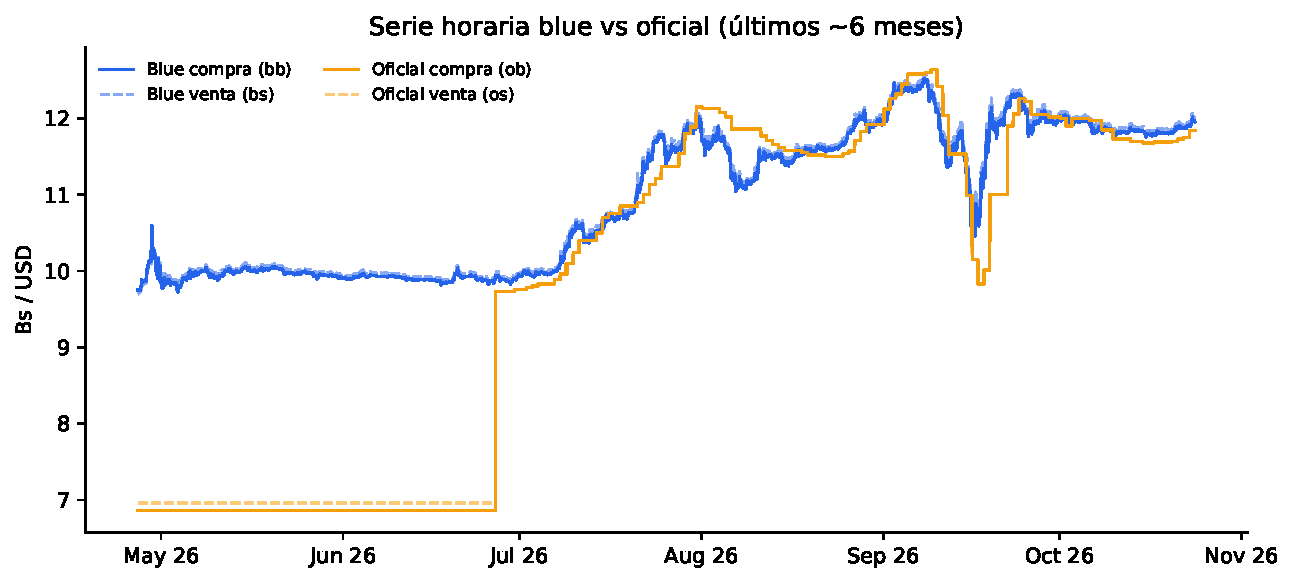
\includegraphics[width=\textwidth]{fig_serie_blue_oficial.pdf}
\caption{Serie por hora blue vs oficial (compra/venta), últimos $\sim$6 meses.}
\label{fig:serie}
\end{figure}

\subsubsection{La brecha cambiaria}

La \hyperref[fig:brecha]{figura~\ref*{fig:brecha}} resume la brecha diaria
(precio medio blue $-$ precio medio oficial) construida desde
\texttt{history\_full.csv} con resampleo diario. Es la base de la variable
objetivo de predicción (Objetivos 1--2, \hyperref[sec:preparacion]{sección~\ref*{sec:preparacion}}).

\begin{figure}[!ht]
\centering
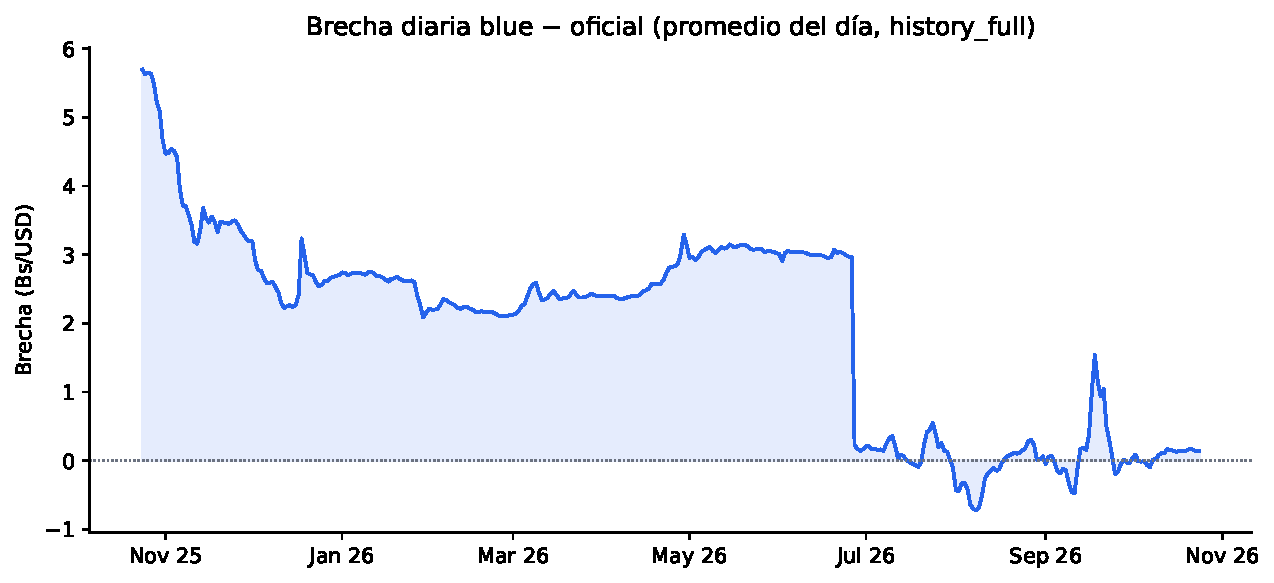
\includegraphics[width=\textwidth]{fig_brecha.pdf}
\caption{Brecha diaria blue $-$ oficial (promedio del día).}
\label{fig:brecha}
\end{figure}

\begin{table}[!ht]
\centering
% Generado por make_figures.py — no editar a mano
\begin{tabular}{@{}lll@{}}
\toprule
Métrica & Valor & Unidad \\
\midrule
Puntos horarios & 4.318 &  \\
Blue medio & 10,98 & Bs/USD \\
Oficial medio & 9,90 & Bs/USD \\
Spread blue medio (bs$-$bb) & 0,05 & Bs/USD \\
Volatilidad diaria blue ($\sigma$ de retornos) & 0,20 & \% \\
Días de brecha (history\_full) & 366 &  \\
Brecha media & 1,94 & Bs/USD \\
Brecha máxima & 5,70 & Bs/USD \\
\bottomrule
\end{tabular}

\caption{Métricas de la serie vigente (blue vs oficial, brecha y
volatilidad).}
\label{tab:resumen}
\end{table}
